\chapter{随机变量及其分布}
\section{随机变量及其分布函数}
\subsection{随机变量}
讨论随机线性的统计规律性,需要我们从数量的角度来研究随机现象,
从而需要在随机试验的可能结果与数之间建立一个对应关系.

许多随机试验的一个可能结果是用一个数来表示的,
这样可在试验结果与数之间建立一个自然的恒等映射.

\begin{definition}
设\(\Omega\)为一试验的样本空间.
如果对每一个样本点\(\omega \in \Omega\),
规定一个实数\(X(\omega)\),
这样就定义了一个定义域为\(\Omega\)的实值函数,
称\(X\)为\DefineConcept{随机变量}(random variable).
通常用大写字母\(X,Y,Z\)等表示随机变量.

一般地,设\(G\)是一个数集,
用\(\Set{\omega \given X(\omega) \in G}\)表示随机变量取值在\(G\)中的样本点构成的事件,
简记为\((X \in G)\),从而该事件的概率可以表示为\(P(X \in G)\).
\end{definition}

\subsection{随机变量的分布函数}
对于概率\(P(X \in G)\),最常见的是\(P(a < X \leq b)\).
而对这一类型的概率,只需求出形如\(P(X \leq x)\)的概率即可,
这是因为\(P(a < X \leq b) = P(X \leq b) - P(X \leq a)\).

\begin{definition}
设\(X\)是一随机变量,对任意实数\(x\),定义\[
	F(x) = P(X \leq x),
	\quad x \in \mathbb{R},
\]
称“\(F\)是随机变量\(X\)的\DefineConcept{分布函数}”.
\end{definition}

\begin{example}
在一个试验中投掷一枚均匀硬币两次,
设随机变量\(X\)表示“试验中出现硬币正面的次数”.
求\(X\)的分布函数\(F(x)\).
\begin{solution}
设硬币正面记作\(H\),反面记作\(T\),那么试验的样本空间为\[
	\Omega = \Set{ HH, HT, TH, TT }.
\]
易见,\(X\)取值为\(0,1,2\),且\(P(X=0) = 1/4\),\(P(X=1) = 1/2\),\(P(X=2) = 1/4\).

当\(x < 0\)时,\(F(x) = P(X \leq x) = P(\emptyset) = 0\);
当\(0 \leq x < 1\)时,\(F(x) = P(X \leq x) = P(X=0) = 1/4\);
当\(1 \leq x < 2\)时,\(F(x) = P(X \leq x) = P(X=0 \lor X=1) = P(X=0)+P(X=1) = 3/4\);
当\(x \geq 2\)时,\(F(x) = P(X \leq x) = P(\Omega) = 1\).

综上所述,\(X\)的分布函数为\[
	F(x) = \left\{ \begin{array}{cl}
		0, & x < 0, \\
		1/4, & 0 \leq x < 1, \\
		3/4, & 1 \leq x < 2, \\
		1, & x \geq 2.
	\end{array} \right.
\]
\end{solution}
\end{example}

\begin{property}
设\(F(x)\)为随机变量\(X\)的分布函数,则
\begin{enumerate}
	\item 当\(x_1 < x_2\)时,有\(F(x_1) \leq F(x_2)\),即\(F(x)\)单调不减;
	\item \(F(-\infty)=P(X \leq -\infty) = \lim_{x \to -\infty}{F(x)} = 0\),
	\(F(+\infty)=P(X \leq +\infty) = \lim_{x \to +\infty}{F(x)} = 1\);
	\item \(F(x)\)是右连续的,即对任意\(x\),有\(F(x^+)=F(x)\);
	\item 对任意\(x_0\),\(P(X=x_0)=F(x_0)-F(x_0^-)\).
\end{enumerate}
\end{property}
需要指出,上述前三点也是分布函数的特征,即任何一个函数只要满足这三点就是某随机变量的分布函数.

\section{离散型随机变量及其分布}
\subsection{离散型随机变量及其分布的概念与性质}
\begin{definition}
若随机变量\(X\)的所有可能取值为有限个或可数无穷多个值,则称\(X\)为\DefineConcept{离散型随机变量}.
\end{definition}

\begin{definition}
设离散型随机变量\(X\)的取值为\(\AutoTuple{x}{n},\dotsc\),
且\(X\)取各值的概率为\[
	p_k = P(X=x_k),
	\quad k=1,2,\dotsc,
\]
称上式为离散型随机变量\(X\)的\DefineConcept{概率分布},
或\DefineConcept{概率函数},
也可称为\DefineConcept{分布律}.
\end{definition}

这样,概率分布刻画了离散型随机变量的统计规律性.

\(X\)的概率分布可用表格或矩阵表示,即
\begin{center}
	\begin{tabular}{c|*5c}
		\hline
		\(X\) & \(x_1\) & \(x_2\) & ... & \(x_n\) & ... \\ \hline
		\(p_k\) & \(p_1\) & \(p_2\) & ... & \(p_n\) & ... \\ \hline
	\end{tabular}
\end{center}
或
\[
	X \sim \begin{pmatrix}
		x_1 & x_2 & \dots & x_n & \dots \\
		p_1 & p_2 & \dots & p_n & \dots
	\end{pmatrix}.
\]

\begin{property}\label{theorem:随机变量及其分布.离散型随机变量的密度函数的性质}
离散型随机变量的概率分布有如下的性质:
\begin{enumerate}
	\item 非负性
	\(p_k \geq 0, \quad k = 1,2,\dots\);

	\item 归一性
	\(\sum_{k}{p_k} = 1\).
\end{enumerate}
\end{property}

这两个性质也是离散型随机变量概率分布的特征,
即对任何一个满足以上两性质的数列\(\{p_k\}\),
都存在一个离散型随机变量\(X\)及数列\(\{x_k\}\),
使得\[
	P(X=x_k) = p_k,
	\quad k=1,2,\dotsc.
\]

易见离散型随机变量的概率分布与分布函数是相互确定的.
当已知概率分布\[
	p_k = P(X=x_k),
	\quad k=1,2,\dotsc,
\]
注意到事件\((X=x_k)\ (k=1,2,\dotsc)\)是两两互斥的,有\begin{equation}
	F(x) = P(X \leq x)
	= P\left[ \bigcup_{x_k \leq x} (X = x_k) \right]
	= \sum_{x_k \leq x} p_k.
\end{equation}

反之,当已知离散型随机变量\(X\)的分布函数\(F(x)\),
则\(X\)的取值点\(x_k\)为\(F(x)\)的间断点,
且\(p_k = P(X=x_k)\)为\(F(x)\)在\(x_k\)处的跃度,
从而可得\(X\)的概率分布.

\subsection{常见离散型分布}

以下几个概率分布是最常见、应用最广泛的离散型随机变量的概率分布,其中二项分布和泊松分布尤为重要.

\subsubsection{几何分布}
\begin{definition}
在\(n\)重伯努利试验中,若试验可一直重复下去,叫做\DefineConcept{可列重伯努利试验}.
\end{definition}

\begin{definition}
若随机变量\(X\)取值为\(1,2,\dotsc\),且\begin{equation}
p_k = P(X=k) = p q^{k-1}, \quad k=1,2,\dotsc,
\end{equation}其中\(0 < p < 1\),\(q = 1-p\),
则称\(X\)服从参数为\(p\)的\DefineConcept{几何分布},
记为\(X \sim G(p)\).
\end{definition}

几何分布的随机变量\(X\)的意义是在可列重伯努利试验中,
事件在前\(X-1\)次试验时不发生而在第\(X\)次试验时发生的概率.

\subsubsection{超几何分布}
\begin{definition}
设\(N\)、\(n\)、\(m\)为正整数,且\(n \leq N\),\(m \leq N\),
若随机变量\(X\)服从分布律\begin{equation}
	p_k = P(X=k) = \frac{C_m^k C_{N-m}^{n-k}}{C_N^n}, \quad k=0,1,\dotsc,n,
\end{equation}
则称\(X\)服从\DefineConcept{超几何分布},
记为\(X \sim H(n,m,N)\),
其中\(n\)、\(n\)、\(m\)为参数.
\end{definition}

超几何分布的随机变量\(X\)的意义是:
假设一个口袋中有红白两种颜色共计\(N\)个球,其中有\(m\)个红球;
现在我们不放回地从袋中取出\(n\)个球,则取出的红球数为\(X\).

\subsubsection{二项分布}
\begin{definition}
若\(X\)取值为\(0,1,\dotsc,n\),且\begin{equation}
P_n(k) = P(X=k) = C_n^k p^k q^{n-k}, \quad k=0,1,\dotsc,n,
\end{equation}其中\(0 < p < 1\),\(q = 1-p\),
则称\(X\)服从\DefineConcept{二项分布},
记为\(X \sim B(n,p)\).

特别地,当\(n = 1\)时,二项分布\(B(1,p)\)称为\DefineConcept{0-1分布},即\[
X \sim \begin{pmatrix} 0 & 1 \\ q & p \end{pmatrix},
\]或写为\[
P(X=k) = p^k q^{1-k}, \quad k=0,1.
\]
\end{definition}

二项分布的随机变量\(X\)的意义是\(n\)重伯努利试验中“成功”的次数.
假设一个口袋中有红白两种颜色共计\(N\)个球,其中有\(m\)个红球;
现在我们有放回地从袋中取出\(n\)个球,则取出的红球数为\(X\).

\begin{example}
一同学参加英语期末考试,进入考场后才发现耳机没有电池,
于是他在听力部分每题4个选项中随机选一个答案作为正确的答案,
求:\begin{enumerate}
	\item 他在20道听力题中一个也没有选对的概率;
	\item 他在20道听力题中至少选对12个的概率.
\end{enumerate}
\begin{solution}
设\(X\)表示他在20个听力题中选对的题目数,
则\(X\)表示20重伯努利试验中“成功”的次数,
即\(X \sim B(20, 1/4)\).
这样所求的概率为\begin{enumerate}
	\item \(P(X=0) = C_{20}^0 \left(\frac14\right)^0 \left(1-\frac14\right)^{20} = 0.003\ 2\).
	\item \(P(X \geq 12) = \sum_{k=12}^{20} \left(\frac14\right)^k \left(1-\frac14\right)^{20-k} = 0.000\ 9\).
\end{enumerate}
\end{solution}
\end{example}

\begin{theorem}
当\(N\)很大时,二项概率与超几何概率有\[
	\frac{C_m^k C_{N-m}^{n-k}}{C_N^n}
	\approx
	C_n^k p^k (1-p)^{n-k}, \quad k=0,1,\dotsc,n,
\]
其中\(p=\frac{m}{N}\).
也就是说,当\(N\)很大时,不放回抽取可视为有放回抽取.
\end{theorem}

\subsubsection{泊松分布}
\begin{theorem}[泊松定理]
设随机变量\(X_n \sim B(n,p_n)\),\(0 < p_n < 1\),且满足\(n p_n = \lambda\),则\begin{equation}
	\lim_{n\to\infty} P(X_n=k)
	= \lim_{n\to\infty} C_n^k p_n^k (1-p_n)^{n-k}
	= \frac{\lambda^k}{k!} e^{-\lambda},
	\quad k=0,1,\dotsc.
\end{equation}
\begin{proof}
因为\begin{align*}
	P(X_n=k) &= C_n^k p_n^k (1-p_n)^{n-k}
	= \frac{1}{k!} n(n-1)\dotsm(n-k+1)
	\left(\frac{\lambda}{n}\right)^k
	\left(1-\frac{\lambda}{n}\right)^{n-k} \\
	&= \frac{1}{k!}
	\cdot \frac{n(n-1)\dotsm(n-k+1)}{n^k}
	\cdot \lambda^k
	\cdot \left(1-\frac{\lambda}{n}\right)^n
	\cdot \left(1-\frac{\lambda}{n}\right)^{-k},
\end{align*}
其中\(\lambda\)是与\(n\)无关的数,
而\(k\)是任意给定的非负整数,
从而\[
	\lim_{n\to\infty} \frac{n(n-1)\dotsm(n-k+1)}{n^k}
	= \lim_{n\to\infty} \frac{n}{n}
	\cdot \lim_{n\to\infty} \frac{n-1}{n}
	\dotsm \lim_{n\to\infty} \frac{n-k+1}{n}
	= 1^k = 1,
\]\[
	\lim_{n\to\infty} \left(1-\frac{\lambda}{n}\right)^{-k}
	= \left(1-\lim_{n\to\infty} \frac{\lambda}{n}\right)^{-k}
	= 1^{-k} = 1,
\]\[
	\lim_{n\to\infty} \left(1-\frac{\lambda}{n}\right)^n
	= \lim_{n\to\infty}
	\left(1-\frac{\lambda}{n}\right)^{\frac{n}{\lambda} \cdot \lambda}
	= e^{-\lambda},
\]
所以\[
	\lim_{n\to\infty} P(X_n=k)
	= \frac{\lambda^k}{k!} e^{-\lambda},
	\quad k=0,1,\dotsc.
	\qedhere
\]
\end{proof}
\end{theorem}

注意到泊松定理中极限值\(\frac{\lambda^k}{k!} e^{-\lambda} > 0\ (k=0,1,\dotsc)\),
且\(\sum_{k=0}^\infty \frac{\lambda^k}{k!} e^{-\lambda} = 1\),
满足非负性和规范性,从而可以据此定义一个分布.

\begin{definition}
若随机变量\(X\)可能的取值为\(0,1,2,\dotsc\),
且\begin{equation}\label{equation:随机变量及其分布.泊松分布的分布律}
	P(X=k) = \frac{\lambda^k}{k!} e^{-\lambda},
	\quad k=0,1,\dotsc,
\end{equation}
其中\(\lambda > 0\)为常数,
则称\(X\)服从泊松分布,
记为\(X \sim P(\lambda)\).
\end{definition}

由泊松定理可见,当\(p\)较小(通常要求\(p \leq 0.1\)),而\(n\)较大(通常要求\(n \geq 50\))时,
二项分布的概率函数近似于泊松分布的概率函数,即\[
	P_n(k) = C_n^k p^k (1-p)^{n-k}
	\approx \frac{\lambda^k}{k!} e^{-\lambda},
	\quad k=0,1,\dotsc,n,
\]
其中\(\lambda = n p\).

\subsubsection{帕斯卡分布}
\begin{definition}
在可列重伯努利试验中,
假设每次试验成功的概率为\(p\ (0<p<1)\).
设\(X\)表示第\(r\)次成功所在的试验次数,
则\begin{equation}
P(X=k) = C_{k-1}^{r-1} p^r (1-p)^{k-r},
\quad k=r,r+1,\dotsc.
\end{equation}
称这个分布为\DefineConcept{负二项分布}或\DefineConcept{帕斯卡分布},
记作\(X \sim NB(r, p)\).
\end{definition}

几何分布\(G(p)\)等价于帕斯卡分布\(NB(1,p)\).

\section{连续型随机变量及其分布}
\subsection{连续型随机变量及其概率密度函数}
\begin{definition}
设随机变量\(X\)的分布函数为\(F(x)\),
若存在一个非负函数\(f(x)\),
使得对任意实数\(x\),有\[
	F(x) = \int_{-\infty}^x f(t) \dd{t},
\]
则称\(X\)为\DefineConcept{连续型随机变量},
\(f(x)\)称为\(X\)的\DefineConcept{概率密度函数},
简称为\DefineConcept{密度函数}或\DefineConcept{密度}.
\end{definition}

\begin{property}\label{theorem:随机变量及其分布.连续型随机变量的密度函数的性质}
密度函数具有以下两个性质:
\begin{enumerate}
	\item 非负性:\(f(x) \geq 0, \quad x \in (-\infty,+\infty)\);
	\item 规范性:\(\int_{-\infty}^{+\infty} f(x) \dd{x} = 1\).
\end{enumerate}
\end{property}
这两个性质也是密度函数的特征,
即若任何一个函数\(g(x)\)具有以上两个性质,
则\(g(x)\)必是某一个连续型随机变量的密度函数.

\begin{theorem}
设\(X\)为连续型随机变量,\(F(x)\)和\(f(x)\)分别为\(X\)的分布函数与密度函数,则
\begin{enumerate}
	\item 对任意常数\(a < b\),有\[
		P(a < X \leq b) = \int_a^b{f(x) \dd{x}};
	\]

	\item 若\(F(x)\)是连续函数,则在\(f(x)\)的连续点\(x_0\)有\[
		F'(x_0) = f(x_0);
	\]

	\item 对任意常数\(C\),有\(P(X=C) = 0\).
\end{enumerate}
\end{theorem}

定理说明连续型随机变量取任意数值的概率都为0,即\[
	P(X=k) = 0.
\]
从而结论1可以表为\[
	P(a < X \leq b)
	= P(a \leq X \leq b)
	= P(a \leq X < b)
	= P(a < X < b)
	= \int_a^b f(x) \dd{x}.
\]
由此可见,一个连续型随机变量\(X\)的密度函数可在有限个点上取值不同,
这样并不影响\(X\)的分布函数,从而密度函数不唯一.

\subsection{常见连续型分布}

\subsubsection{均匀分布}
\begin{definition}
设随机变量\(X\)的密度函数为\begin{equation}
	f(x) = \left\{ \def\arraystretch{1.5}
	\begin{array}{cl}
		\frac{1}{b-a}, & x \in (a,b), \\
		0, & x \in (-\infty,a) \cup (b,+\infty), \\
	\end{array} \right.
\end{equation}
则称\(X\)在区间\([a,b]\)上服从\DefineConcept{均匀分布},
记为\(X \sim U(a,b)\),
其中\(a < b\).

一般地,把密度函数大于0的区间叫做连续型随机变量的取值区间.
\end{definition}

\begin{theorem}
均匀分布的分布函数为\begin{equation}
	F(x) = \left\{ \def\arraystretch{1.5}
	\begin{array}{cl}
		0, & x < a, \\
		\frac{x-a}{b-a}, & a \leq x \leq b, \\
		1, & x > b. \\
	\end{array} \right.
\end{equation}
\end{theorem}

\subsubsection{指数分布}
\begin{definition}
设随机变量\(X\)的密度函数为\begin{equation}
f(x) = \left\{ \def\arraystretch{1.5}
\begin{array}{cl}
\lambda e^{-\lambda x}, & x > 0, \\
0, & x \leq 0, \\
\end{array} \right.
\end{equation}其中\(\lambda > 0\)为常数,
则称“\(X\)服从\DefineConcept{指数分布}”,
记为\(X \sim e(\lambda)\).
\end{definition}

\begin{theorem}
指数分布的分布函数为\begin{equation}
	F(x) = \left\{ \def\arraystretch{1.5}
	\begin{array}{cl}
		1 - e^{-\lambda x}, & x > 0, \\
		0, & x \leq 0. \\
	\end{array} \right.
\end{equation}
\end{theorem}

\begin{theorem}[指数分布的无记忆性]
对于任意\(t > 0\),\(\tau > 0\),当\(X \sim e(\lambda)\)时,有\[
P(X > t + \tau \vert X > t) = P(X > \tau).
\]

指数分布是唯一具有无记忆性的连续性分布.
\end{theorem}

\subsubsection{\textGamma 分布}
\begin{definition}
若随机变量\(X\)有密度函数\begin{equation}
	f(x) = \left\{
	\def\arraystretch{1.5}
	\begin{array}{cl}
		\frac{\beta^\alpha}{\Gamma(\alpha)} x^{\alpha-1} e^{-\beta x}, & x > 0, \\
		0, & x \leq 0, \\
	\end{array} \right.
\end{equation}
其中\(\alpha\)、\(\beta\)是正常数,
则称“\(X\)服从 \DefineConcept{\(\Gamma\)分布}”,
记为\(X \sim \Gamma(\alpha,\beta)\).
%@see: https://mathworld.wolfram.com/GammaDistribution.html
\end{definition}

指数分布\(e(\lambda)\)等价于\(\Gamma\)分布\(\Gamma(1,\lambda)\).

\begin{figure}[ht]
	\centering
	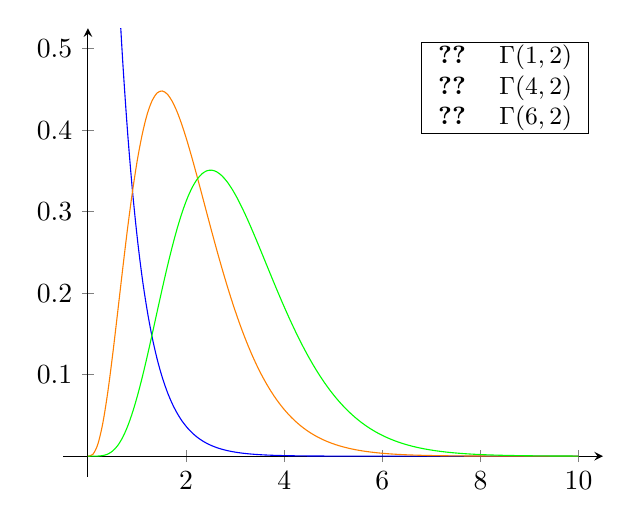
\begin{tikzpicture}
		\begin{axis}[
			name=GammaDistribution,
			axis y line=middle,
			axis x line=middle,
			enlarge x limits=0.05,
			enlarge y limits=0.05,
			ymax=.5,
			ymin=0,
		]
			\def\plotGDPDF#1#2#3{\addplot[color=#3,samples=100,smooth,domain=0:10]{%定义
				(2^(#1))*(x^(#1-1))*exp(-2*x)/(#2)
			}}%
			\plotGDPDF{1}{1}{blue};\label{pgfplots:伽马分布.Gamma(1,2)}
			\plotGDPDF{4}{6}{orange};\label{pgfplots:伽马分布.Gamma(4,2)}
			\plotGDPDF{6}{120}{green};\label{pgfplots:伽马分布.Gamma(6,2)}
		\end{axis}
		\node[draw,fill=white,inner sep=0pt,below left=0.5em]
		at(GammaDistribution.north east){\small\begin{tabular}{cl}
			\ref{pgfplots:伽马分布.Gamma(1,2)} & \(\Gamma(1,2)\) \\
			\ref{pgfplots:伽马分布.Gamma(4,2)} & \(\Gamma(4,2)\) \\
			\ref{pgfplots:伽马分布.Gamma(6,2)} & \(\Gamma(6,2)\) \\
		\end{tabular}};
	\end{tikzpicture}
	\caption{\(\Gamma\)分布的密度函数}
	% Mathematica: Plot[Table[PDF[GammaDistribution[\[Alpha], .5], x], {\[Alpha], {1, 4, 6}}] // Evaluate, {x, 0, 20}, PlotRange -> {0, .5}, Filling -> Axis]
\end{figure}


\begin{definition}
若一个元件或系统的寿命\(X\)满足一个连续型分布,\(X \sim F(t)\),
则其可靠度函数定义为\[
R(t) = 1 - F(t) = P(X > t).
\]其失效率函数定义为\[
r(t) = \frac{f(t)}{R(t)}.
\]

当\(\increment t\)较小时,\(r(t) \increment t\)表示元件或系统在时刻\(t\)以前正常工作,
但在时间\((t,t+\increment t)\)失效的概率.
\end{definition}

注意,当\(\alpha = 1\)时,\(\Gamma\)分布\(\Gamma(1,\beta)\)为指数分布\(e(\beta)\),即系统失效概率不随时间变化;
当\(0 < \alpha < 1\)时,系统失效概率随时间\(t\)增加呈下降趋势;而当\(\alpha > 1\)时则正相反.

\section{随机变量函数的分布}
在实际应用中,常常遇到随机变量的函数.
如一个圆柱状工件的半径为\(X\),则工件截面积为\(\pi X^2\).
一般地,随机变量\(X\)的函数\(Y=g(X)\)是一个样本空间到实数域的复合函数,所以\(Y\)也是随机变量.
因此有依据\(X\)的分布求出\(Y\)的分布的问题.
这样的问题在离散的情形下较为简单,在连续的情形下较为复杂.

\subsection{求解离散型随机变量函数的概率分布的基本方法步骤}
设随机变量\(X\)的概率分布为\(p_k = P(X = x_k)\ (k=1,2,\dotsc)\),
则\(Y = g(X)\)的概率分布为\[
P(Y = y_j) = \sum_{g(x_k) = y_j} p_k
\quad(j=1,2,\dotsc).
\]

\begin{example}
设随机变量\(X\)的概率分布为\[
X \sim \begin{pmatrix}
-1 & 0 & 1 & 2 \\
0.2 & 0.3 & 0.3 & 0.2
\end{pmatrix},
\]\(Y=X^2\),\(Z=\frac{X^3+1}{2}\),求\(Y,Z\)的概率分布.
\begin{solution}
由于\(X\in\{-1,0,1,2\}\),所以\(Y\in\{0,1,4\}\),\begin{align*}
P(Y=0) &= P(X=0) = 0.3, \\
P(Y=1) &= P(X=-1 \lor X=1) \\
	&= P(X=-1) + P(X=1)
	= 0.5, \\
P(Y=4) &= P(X=2) = 0.2,
\end{align*}
从而\[
Y \sim \begin{pmatrix}
0 & 1 & 4 \\
0.3 & 0.5 & 0.2
\end{pmatrix}.
\]

同理,\(Z\in\Set{0,\frac{1}{2},1,\frac{9}{2}}\),且\begin{align*}
P(Z=0) &= P(X=-1) = 0.2, \\
P(Z=1/2) &= P(X=0) = 0.3, \\
P(Z=1) &= P(X=1) = 0.3, \\
P(Z=9/2) &= P(X=2) = 0.2,
\end{align*}
从而\[
Z \sim \begin{pmatrix}
0 & \frac{1}{2} & 1 & \frac{9}{2} \\
0.2 & 0.3 & 0.3 & 0.2
\end{pmatrix}.
\]
\end{solution}
\end{example}

\subsection{求解连续型随机变量函数的密度函数的基本方法步骤}
设随机变量\(X\)的密度函数为\(f_X(x)\),
要求\(Y = g(X)\)的密度函数,
\begin{enumerate}
	\item 首先依据\(X\)的取值区间,
	求出\(Y\)的值域\(R(Y)\).

	\item 然后求出\(Y\)的分布函数,
	即对\(\forall y \in R(Y)\),
	有\[
		F_Y(y) = P(Y \leq y)
		= P[g(X) \leq y]
		= P[X \in G(y)]
		= \int_{G(y)} f_X(x) \dd{x},
	\]
	其中\(G(y) = \Set{ x\in\mathbb{R} \given g(x) \leq y }\).
	对\(\forall y \notin R(Y)\),
	有\[
		F_Y(y) = 0
		\quad\text{或}\quad
		F_Y(y) = 1.
	\]

	\item 对\(Y\)的分布函数求导,得\[
		f_Y(y) = \left\{ \begin{array}{cl}
			F_Y'(y), & y \in R(Y), \\
			0, & y \notin R(Y).
		\end{array} \right.
	\]
\end{enumerate}
